%%%%%%%%%%%%%%%%%% CALCULUS ON MANIFOLDS

\chapter{Calculus on Manifolds}

\section{What is a Manifold?}

A $m$-dimensional {\sc Manifold} is a (topological) space which at each point looks locally like $\R^m$. Note that $m$ is a fixed number, and defines the dimension of the manifold.

\begin{Def}[Manifold]
  A {\sc Manifold}\index{Manifold}, $M$, is a topological space homeomorphic to $\R^m$.
\end{Def}



Examples of manifolds are  the body of a cylinder,  the spheres ($S^m$), the torus ($T^m$).

%% \begin{center}
%%   \begin{tikzpicture}[baseline]
%%     \begin{axis}[hide axis,axis equal=true,]
%%     \addplot3[  
%%       surf, shader=interp,
%%       unit vector ratio=1 1 1,
%%       colormap/greenyellow,
%%       %mesh,
%%       fill=white,      
%%       point meta=x,
%%       samples=20,
%%       samples y=40,
%%       domain=0:180,
%%       y domain=0:360,
%%     ] (                                                                         
%%              {sin(x)*cos(y)},                                                   
%%              {sin(x)*sin(y)},                                                   
%%              {cos(x)}                                                           
%%    );          
%%     \end{axis}
%%   \end{tikzpicture}
%%   \hspace{1cm}
%%   \begin{tikzpicture}[baseline]
%%     \begin{axis}
%%       [
%%         hide axis,
%%         %view={60}{30},
%%         axis equal image,
%%       ]
%%       \addplot3 [
%%         surf, shader=interp,
%%         point meta=x,
%%         colormap/greenyellow,
%%         samples=40,
%%         samples y=20,
%%         z buffer=sort,
%%         domain=0:360,
%%         y domain=0:360
%%       ] (
%%                 {(3.5 + 0.5*cos(y))*cos(x)},
%%                 {(3.5 + 0.5*cos(y))*sin(x)},
%%                 {0.5*sin(y)});
%%       \addplot3 [
%%         samples=40,
%%         samples y=1,
%%         domain=0:360,
%%         thick
%%       ] (
%%                 {(3.5 + 0.5*cos(80))*cos(x)},
%%                 {(3.5 + 0.5*cos(80))*sin(x)},
%%                 {0.5*sin(80)});
%%     \addplot3 [
%%       samples=10,
%%       samples y=1,
%%       domain=-65:130,
%%       thick
%%     ] (
%%               {3.5 + 0.5*cos(x)},
%%               {0},
%%               {0.5*sin(x)});
%%     \end{axis}
%%   \end{tikzpicture}
%% \end{center}
\begin{center}
  \begin{tabular}{cc}
    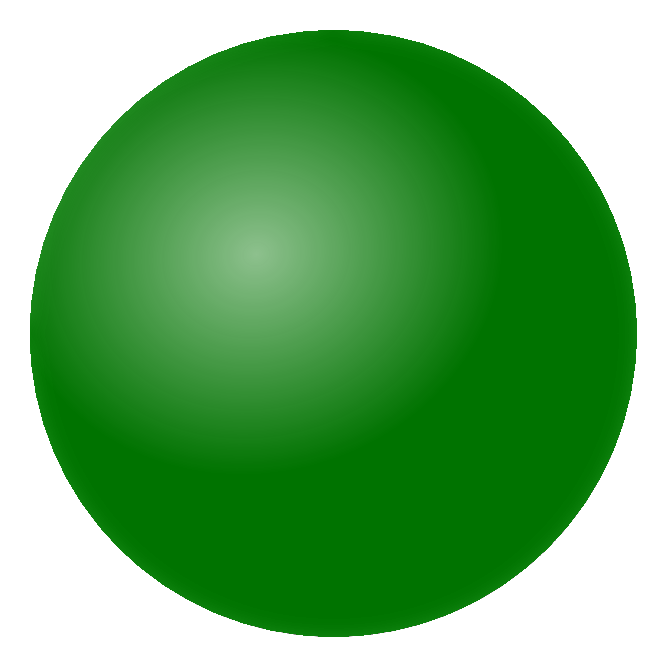
\includegraphics[scale=.4]{Pict/Sphere2.pdf}  & 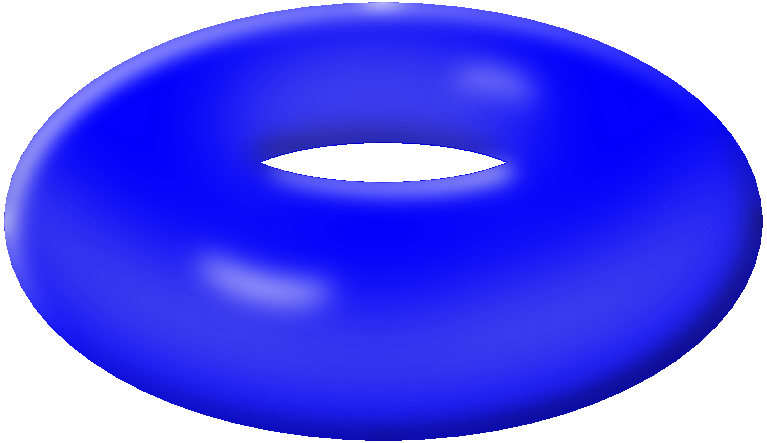
\includegraphics[scale=.4]{Pict/Torus.pdf}
  \end{tabular}
\end{center}
%% \begin{figure}[H]
%%   \begin{center}
%%      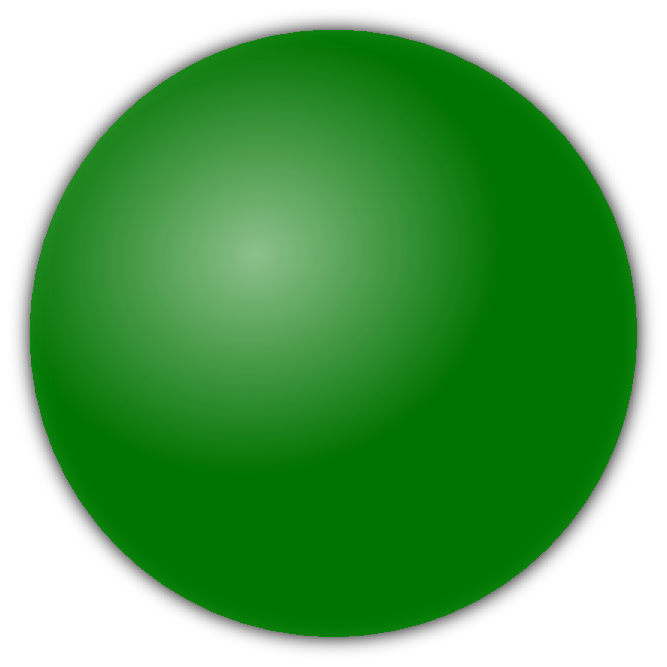
\includegraphics[scale=.4]{Pict/Sphere.pdf} 
%%      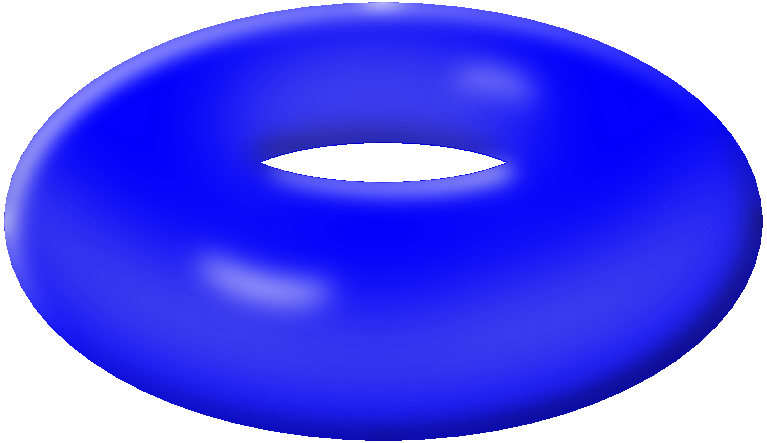
\includegraphics[scale=.4]{Pict/Torus.pdf}
%%   \end{center}
%%   \caption{Examples of manifolds}
%% \end{figure}


More illustrative is an example of a non-manifold, such as the body of a cone. A cone is not a manifold because the neighbourhood of the apex looks not line $\R^2$.
\begin{center}
  \begin{tikzpicture}[scale=1.5,
      spy using outlines={circle, magnification=6, size=2.5cm,connect spies}] 

    \pgfmathsetmacro{\a}{3}
    \pgfmathsetmacro{\b}{5}
    \pgfmathsetmacro{\th}{30}
    \pgfmathsetmacro{\ph}{atan(\a * tan(\th) / \b)}
    \pgfmathsetmacro{\r}{\a * tan(\th)}
    \pgfmathsetmacro{\h}{sqrt(\a*\a +\r*\r)}
    \pgfmathsetmacro{\H}{sqrt(\b*\b +\r*\r)}

    \coordinate (O) at (0,0);
    \coordinate (X) at (0,{\b-\a});

    \draw[thick,dashed] (X)  +(270+\th:\h) arc (90-\ph:90+\ph:\H);
    \shadedraw[left color=blue, right color= blue!60!black, middle color=blue!60!white, shading angle={90-\th}, opacity=.7] (X) -- +(270-\th:\h) arc (270-\ph:270+\ph:\H) --cycle;
    

    \spy on (X) in node at (5,1);
  \end{tikzpicture}
\end{center}

\section{Geometrical Objects on Manifolds}

The trick to define geometrical objects on  manifolds, $M$, is to find a way to assign an analog to the object defined on $\R^m$. This is achieved by the following procedure:
\begin{itemize}
\item Given a manifold $M$, set a point $p\in M$ and consider the neighbourhood, $U$, of $p$. The point is represented in the figure below by a black dot, while the neighbourhood $U$ is limited by a dotted circle around $p$.
\item For each choice of $U$, one can find a map from $M$ to $\R^m$, $\varphi:M\to \R^m$, called a chart on $U$.
\item Then, the $\varphi$ map helps to associate equivalent geometrical quantities on $M$ to those on $\R^m$.
\end{itemize}
\begin{center}
  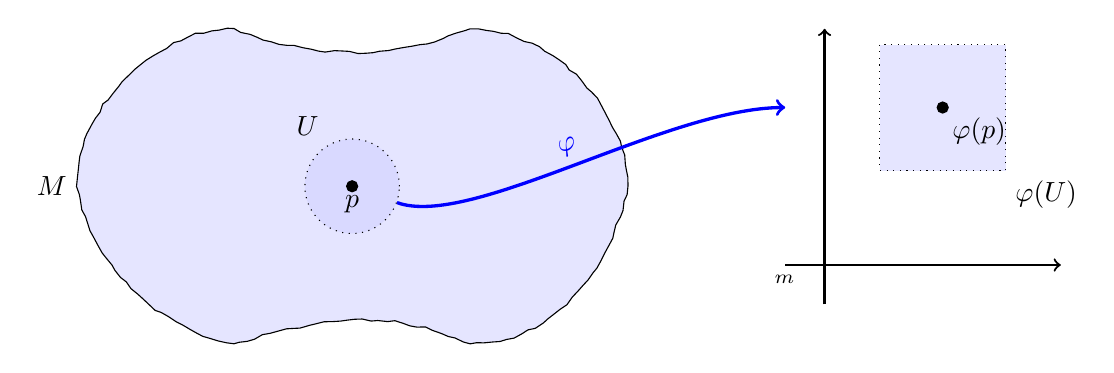
\begin{tikzpicture}
    \coordinate (P) at (3.5,0);
\draw[draw=black,
  fill = blue!10,
  decoration={random steps,segment length=1mm,amplitude=.5pt},
  decorate,
  %rounded corners
  ]
(0,0) .. controls (0,1) and (1,2) .. (2,2) .. controls (3,1.6) and (4,1.6) .. (5,2) ..controls (6,2) and (7,1) .. (7,0) ..controls (6.8,-1) and (6.1,-2) .. (5,-2) .. controls (3.8,-1.5) and (3.1,-1.7) .. (2,-2) ..controls (1,-1.8) and (0.2,-1) .. (0,0) node[anchor=east] {$M$} -- cycle;
%% \draw[thick,red, dashed] (2,-1)  ..controls (3,1) and (4,-1) .. (5,1);

\node[draw, dotted, fill = blue!15, circle, minimum size=1.2cm,label=120:$U$] (ball) at (P) {};
\draw[fill=black] (P) node[anchor= north] {$p$} circle (2pt);

\draw[blue,very thick,->] (node cs:name=ball,angle=-20) .. controls +(-20:1cm) and (7.5,1) .. node[midway, above,sloped] {$\varphi$} (9,1);
\draw[thick,->] (9,-1) node[anchor=north] {$\R^m$} -- (12.5,-1);
\draw[thick,->] (9.5,-1.5) -- (9.5,2);

\draw[fill = blue!10,dotted] (10.2,1.8) rectangle (11.8,0.2) node[anchor= north west] {$\varphi(U)$};
\draw[fill=black] (11,1) node[anchor= north west] {$\varphi(p)$} circle (2pt);

  \end{tikzpicture}
\end{center}

From the procedure described, one can guess that a scalar field on $M$ is an assignment of a scalar to every point $p\in M$. The only non-trivial consideration is that the assignation must be consistent, i.e., the scalar should be independent of the chart one choose to map $M$ to $\R^m$. On $S^1$, the ``consistency'' condition is that one you go all around the sphere, the number you get must be the same that the one you begun with.

\subsection{Vectors}

On Euclidean geometry, one defines the ``velocity'' vector as the derivative of the position with respect to the time. This definition can be generalised to every curve, $c$, of a parameter $t$ over the Euclidean space, i.e., $c:\R\to\R^m$ defined by $c: t\to c(t)$.

Moreover, the space the function is mapped to could be a manifold instead of $\R^m$. Therefore, a \idx{curve} on $M$ is a (continuous) map $c:\R\to M$. This is represented in the figure by the \textcolor{red}{red map}, and its image is the {\color{red} red dotted line}.

\begin{center}
  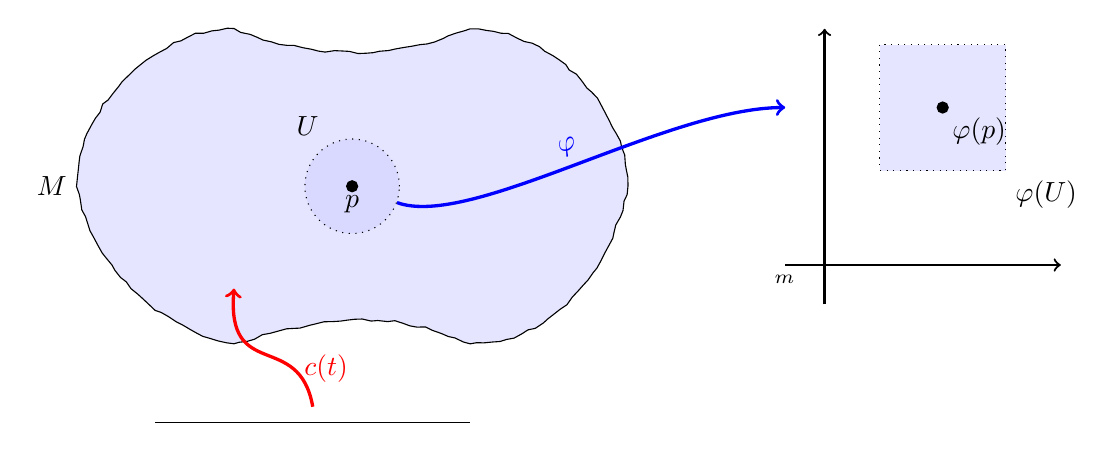
\begin{tikzpicture}
    \coordinate (P) at (3.5,0);
\draw[draw=black,
  fill = blue!10,
  decoration={random steps,segment length=1mm,amplitude=.5pt},
  decorate,
  %rounded corners
  ]
(0,0) .. controls (0,1) and (1,2) .. (2,2) .. controls (3,1.6) and (4,1.6) .. (5,2) ..controls (6,2) and (7,1) .. (7,0) ..controls (6.8,-1) and (6.1,-2) .. (5,-2) .. controls (3.8,-1.5) and (3.1,-1.7) .. (2,-2) ..controls (1,-1.8) and (0.2,-1) .. (0,0) node[anchor=east] {$M$} -- cycle;
%% \draw[thick,red, dashed] (2,-1)  ..controls (3,1) and (4,-1) .. (5,1);

\node[draw, dotted, fill = blue!15, circle, minimum size=1.2cm,label=120:$U$] (ball) at (P) {};
\draw[fill=black] (P) node[anchor= north] {$p$} circle (2pt);

\draw[blue,very thick,->] (node cs:name=ball,angle=-20) .. controls +(-20:1cm) and (7.5,1) .. node[midway, above,sloped] {$\varphi$} (9,1);
\draw[thick,->] (9,-1) node[anchor=north] {$\R^m$} -- (12.5,-1);
\draw[thick,->] (9.5,-1.5) -- (9.5,2);

\draw[fill = blue!10,dotted] (10.2,1.8) rectangle (11.8,0.2) node[anchor= north west] {$\varphi(U)$};
\draw[fill=black] (11,1) node[anchor= north west] {$\varphi(p)$} circle (2pt);

    \draw (1,-3) node[anchor=east] {$\R$} -- (5,-3);
    \draw[very thick, red,->] (3,-2.8) .. controls +(100:1cm) and (1.9,-2.5).. node[anchor=west,near start] {$c(t)$} (2,-1.3);
  \end{tikzpicture}
\end{center}

Consider a map $f:M\to \R$, and restrict the domain of $f$ to the points $c(t)\in M$. Then the derivative of $f$ yields
\begin{align}
  f'\(c(t)\)&= \pder{f}{x^\mu}\pder{x^\mu}{t}\notag\\
  &= X[f],
\end{align}
where $X$ is the object one would like to call a \emph{vector} on $M$, and is defined through
\begin{align}
  X \equiv X^\mu \pder{}{x^\mu}= \pder{x^\mu}{t}\pder{}{x^\mu},
  \label{def-vector}
\end{align}
and $x^\mu$ are the coordinated of the point $p$ given by the function $c(t)$.
The quantities $X^\mu$ are the components of the vector, while $\pder{}{x^\mu}\equiv \pa{\mu}$ are the basis of the vector.

Note that the definition of the vector $X$ through Eq.~\eqref{def-vector}, is independent of the function $f$, thus is a well-defines quantity. Additionally, the definition could be done with an arbitrary coordinate system $y^\mu = \Lambda^\mu{}_\nu x^\nu$, and the definition would give the same. Therefore, the components of the vector transforms as the coordinate, while the basis transform with the inverse transformation,
\begin{align}
  \pder{}{y^\mu} &= \(\Lambda^{-1}\)_\mu{}^\nu\pder{}{x^\nu},\\
  {X'}^\mu &= \Lambda^\mu{}_\nu X^\nu.
\end{align}

From the definition, one expect that the vectors  lie on a \emph{tangent space}\index{space!tangent} to the point $p$, this space is denoted by $T_p M$. When the manifold is not flat, the tangent spaces  at $p$ and at $q$ are not necessary the same, thus, when one want to specify a vector a total of $2m$ coordinates are needed, $m$ of them to denote the point $p\in M$ and the other $m$ to denote the vector on $T_p M$.

Therefore, in order to define vector fields on $M$, the natural structure to consider is the disjoint union of all the tangent spaces. This structure is call the \emph{tangent bundle}\index{bundle!tangent}, $TM$, and mathematically is defined as
\begin{align}
  TM = \coprod_{p\in M} T_p M.
\end{align}
From the above arguments, it is clear that $\dim(TM)=2m$.


\subsection{One-Forms}

Given a vector $V\in T_p M$, one might define a linear application $\omega:T_p M\to \R$, in a way that
\begin{align}
  V[f] = V^\mu\pa{\mu}f\equiv \bk{\de{f}}{V}\in \R.
\end{align}
Above, bracket $\bk{\bullet}{\bullet}$ denotes the inner product, and $\de{f}$ is a \emph{1-form}, i.e., a linear application from a vector into the reals.

The 1-form $\de{f}$ can be expanded in components,
\begin{align}
  \de{f} = \pder{f}{x^\mu}\de{x^\mu},
\end{align}
with basis of the dual vector space $\de{x^\mu}$. The basis of the dual space can be chosen to satisfy,
\begin{align}
  \bk{\de{x^\mu}}{\pa{\nu}} = \delta^\mu_\nu.
\end{align}

Clearly 1-forms lie on a vector space, $T^*_p M$, called the dual vector space or \emph{cotangent space}\index{space!cotangent}. As before, one defines the structure where 1-form fields live, as 
\begin{align}
  T^*M = \coprod_{p\in M} T^*_p M,
\end{align}
called \emph{cotangent bundle}\index{bundle!cotangent}, just like before, $\dim(T^*M)=2m$.

\subsection{Tensors}

Tensors\index{Tensor} are multi-linear objects, and they can be expressed in a ``vector basis'' given by the tensor product of basis of either $TM$ or $T^*M$. The tensor product is denoted by $\otimes$, and  it multiplies the basis of ``vector'' spaces in a way they transform independently. 

Tensors are said to be of type $\binom{p}{q}$\index{Tensor!type} if it can be expanded in a basis containing the tensor product of $p$ times the basis of $T_xM$ and $q$ times the basis of $T_x^*M$, i.e.,  $\binom{p}{q}$-tensors lie on 
\begin{equation}
  \Te[p][q]{M} = \(\otimes^p T_x M\) \otimes \(\otimes^q T_x^*M\).
\end{equation}
Additionally, the rank of the tensor\index{Tensor!rank} corresponds to the ``number of indices'', i.e., if $T \in \Te[p][q]{M} $ its rank is $p+q$.

\begin{Ebox}
  How do the components of $T$ transform? Where 
  \begin{align}
    T = T^{a_1 \cdots a_p}{}_{b_1 \cdots b_q} \partial_{a_1} \otimes \cdots \otimes \partial_{a_p} \otimes \de{x}^{b_1} \otimes \cdots \otimes \de{x}^{b_q}.
  \end{align}
\end{Ebox}



\section{Induced Maps and Submanifolds}

Given a map, $f$, between two manifolds, $f:M\to N$, there are induced maps\index{map!induced} on all of the geometrical structures defined over them. Below, two important cases are considered, to know, the differential map and the pullback.

\subsection{Differential Map}

Let $f$ be a map from $M$ to $N$, $f:M\to N$. Then, the \emph{differential map}\index{map!differential} or \emph{push-forward}\index{push-forward}
\begin{align*}
  f_*:T_p M\to T_{f(p)}N,
\end{align*}
is such that,
\begin{align}
  \(f_* V\)[g] = V[g\circ f],
\end{align}
for $g$ a function on $N$.

\begin{center}
  \begin{tikzpicture}%[scale=.8]
    \coordinate (P) at (3.5,0);
    \coordinate (fP) at (12.5,0);
    \coordinate (M) at (3.5cm, 3cm);
    \coordinate (N) at (12 cm, 3cm);
    
    \draw[draw=black,
      fill = blue!20,
      decoration={random steps,segment length=1mm,amplitude=.5pt},
      decorate]
    (0,0) .. controls (0,1) and
    (1,2) .. (2,2) .. controls (3,1.6) and
    (4,1.6) .. (5,2) ..controls (6,2) and
    (7,1) .. (7,0) ..controls (6.8,-1) and
    (6.1,-2) .. (5,-2) .. controls (3.8,-1.5) and
    (3.1,-1.7) .. (2,-2) ..controls (1,-1.8) and
    (0.2,-1) .. (0,0)  -- cycle;
    

    \draw[thick,red, dashed] (2,-1)  ..controls (3,1) and (4,-1) .. (5,1);
    \draw[fill=black] (P) node[anchor= north west] {$p$} circle (2pt);
    \node[draw, dotted, circle, minimum size=1.2cm,label=120:$U$] (ball1) at (P) {};

    \draw[draw=black,
      fill = blue!20,
      decoration={random steps,segment length=1mm,amplitude=0.8pt},
      decorate]
    (12,0) ellipse (3.5cm and 2cm);
    \draw[thick,red, dashed] ($(fP) + (-1,-1)$)  ..controls ($(fP) + (-1,0)$) and ($(fP) + (1,0)$) .. ($(fP) + (1,1)$);
    \node[draw, dotted, circle, minimum size=12mm,label=120:$f(U)$] (ball2) at (fP) {};
    \draw[fill=black] (fP) node[anchor= north west] {$f(p)$} circle (2pt);

    \node at (M) {$M$};
    \node at (N) {$N$};
    \draw[blue,very thick,->] ($(M) + (.5cm,0)$) -- node[midway, above,sloped] {$f$} ($(N) + (-0.5cm,0)$);


    \draw[very thick,green!50!black,->] (P) to +(.7,0) node[anchor=west] {$V$};
    \draw[very thick,green!50!black,->] (fP) to +(33:.7cm) node[anchor=south west] {$f_* V$};
    \draw[blue,very thick,->,] (node cs:name=ball1,angle=-20)  to [bend right] node[midway, above,sloped] {$f_*$} (node cs:name=ball2,angle=200);
    
  \end{tikzpicture}
\end{center}

\subsection{Pullback Map}

In the same spirit that the differential map, the map between manifolds $f:M\to N$, induces a relation between the cotangent bundles $T^*M$ and $T^*N$. This action is called \emph{pullback}\index{pullback} and is denoted by $f^*$, where
\begin{equation}
  f^*: T^*_{f(p)}N \to T^*_p M.
\end{equation}

Since the tangent and cotangent spaces are related by the definition of an inner product, $\bk{\bullet}{\bullet}$, the action of the pullback is defined by 
\begin{equation}
  \bk{f^*\omega}{V} = \bk{\omega}{f_*V},
\end{equation}
where $V \in TM$ and $\omega \in T^*N$.

\begin{Ebox}
  Let $M$, $N$ and $P$ be manifolds, and $ f:M\to N$, $g:N\to P$,  be maps between manifolds. 

  Show
  \begin{align*}
    (g\circ f)_* &= g_*\circ f_*\\
    (g\circ f)^* &= f^*\circ g^*
  \end{align*}
\end{Ebox}

\section{Submanifolds}

Submanifolds are restrictions of a manifold, which satisfy the conditions of manifold by themselves. Submanifolds can be defined as maps, $f:M \to N$.

\begin{Def}[Immersion, embedding, submanifold]
  Let $f:M\to N$ be a smooth map and let $\dim(M)\leq \dim(N)$.
  \begin{itemize}
  \item The map $f$ is called an \emph{immersion}\index{immersion} of $M$ into $N$ if its differential map \mbox{$f_*:T_p M\to T_{f(p)}N$} is an injection.
  \item The map $f$ is called an \emph{embedding}\index{embedding} of $M$ into $N$ if $f$ is an injection and an immersion.
  \end{itemize}
  If $f$ is an embedding of $M$ into $N$, the image $f(M)\subset N$ is a \emph{submanifold}\index{submanifold} of $N$.
\end{Def}

\begin{center}
  \begin{tikzpicture}
    \coordinate (O) at (0,0);
    \coordinate (S) at (-4,2);
    \coordinate (fS) at (3,2);

    \pgfmathsetmacro{\r}{1}
    \pgfmathsetmacro{\rx}{2}
    \pgfmathsetmacro{\ry}{1}
    \pgfmathsetmacro{\th}{30}

    \draw[blue,thick] (S) circle [radius=\r cm];
    \node at ($(S)+(75:1.5cm)$) {$S^1$};
    \draw[thick,<->] (0,4) node[anchor=south west] {$\R^2$} -- (O) -- (4,0);
    \draw[blue,thick] (fS) .. controls (5,6) and (6,1) .. (fS) .. controls (1,3) and (0,-2) .. (fS); 

    \draw[red,very thick,->,bend left=30] ($(S)+(45:1.5cm)$) to  node[midway, above,sloped] {$f$}  ($(fS)+(135:1.5cm)$);
  \end{tikzpicture}
\end{center}

\begin{center}
  \begin{tikzpicture}
    \coordinate (O) at (0,0);
    \coordinate (S) at (-4,2);
    \coordinate (gS) at (3,2);

    \pgfmathsetmacro{\r}{1}
    \pgfmathsetmacro{\rx}{2}
    \pgfmathsetmacro{\ry}{1}
    \pgfmathsetmacro{\th}{30}

    \draw[blue,thick] (S) circle [radius=\r cm];
    \node at ($(S)+(75:1.5cm)$) {$S^1$};
    \draw[thick,<->] (0,4) node[anchor=south west] {$\R^2$} -- (O) -- (4,0);
    \draw[blue,thick] (gS) circle [x radius=\rx cm, y radius=\ry cm, rotate=\th];    

    \draw[red,very thick,->,bend left=30] ($(S)+(45:1.5cm)$) to  node[midway, above,sloped] {$g$}  ($(gS)+(135:1.5cm)$);
  \end{tikzpicture}
\end{center}

From the figures above, one notices that both $f$ and $g$ are immersions of $S^1$ into $\R^2$ because each  vector on $TS^1$ posses a unique corresponding vector on either $T\R^2$. However, the map $f$ is not an injection because the cross-path in $f(S^1)$ has not a unique point on $S^1$, therefore, $f$ is not an embedding of $S^1$ into $\R^2$. On the other hand, $g$ is an embedding and its image $g(S^1)\subset \R^2$ is a submanifold of $\R^2$.

\section{Flows and Lie Derivative}

\subsection{Vector Flows}

\subsubsection*{Pictorial Image}

A vector field is a relation that assign a vector to each point of the space. One can imagine a vector field as the set of velocities of a river basin for a given position. If one throws an almost massless piece of paper, the motion of the paper is determined by the velocities of the neighbourhood at its position.

One could say that the position of the piece of paper at a given time, denoted by $x(t)$, is determined by the (vector field of) velocities of the river, denoted by $V$, as follows
\begin{equation}
  \der{x(t)}{t} = V[x(t)].
\end{equation}

\subsubsection*{Mathematically}

Let $V$ be  vector field  on a manifold $M$, and $\sigma$ a map  \mbox{$\sigma:\R\times M\to M$}, satisfying
\begin{equation}
  \der{}{t}\sigma(t,x) = V[\sigma(t,x)],
  \label{eq:flow}
\end{equation}
for every $t\in \R$ and $x\in M$. The map $\sigma$ is said to be the \emph{flow}\index{flow} generated by the vector $V$ on $M$.

From the theory of differential equations, it is evident that to determine a unique solution of Eq.~\eqref{eq:flow}, an initial point, $x_0$, and `time', $t_0$, are needed.

For a fixed point $x_0\in M$, the curve $\sigma(t,x_0)$ is called the \emph{integral curve}\index{curve!integral}
of $V$ at $x_0$.


\begin{WEbox}[%
    frametitle={Finding the integral curve},
    frametitlerule=true,
    frametitlealignment=\centering,
    frametitleaboveskip=10pt,]
  Let $V = x \partial_y - y \partial_x$ be a vector field on $\R^2$. A flow $\sigma:\R\times \R^2 \to \R^2$ is a point in $\R^2$ characterised by the coordinates $x(t)$ and $y(t)$, i.e.,
  \begin{equation}
    \sigma(t,(x,y)) = x(t) \pa{x} + y(t) \pa{y}.
  \end{equation}
  Therefore, the integral curve passing by a point $(x_0,y_0)$ solves the differential equation~\eqref{eq:flow} with the condition
  \begin{equation*}
    \sigma(t_0,(x,y)) = x_0 \pa{x} + y_0 \pa{y}.
  \end{equation*}

  From Eq.~\eqref{eq:flow}, one obtain 
  \begin{align*}
    \der{}{t}\sigma(t,(x,y)) &= V[\sigma(t,(x,y))] \\
    \dot{x}(t) \pa{x} + \dot{y}(t) \pa{y} &= -y(t) \pa{x} + x(t) \pa{y},
  \end{align*}
  or equivalently (due to the orthogonality of the vector basis),
  \begin{align*}
    \dot{x}(t) &= -y(t),  \\
    \dot{y}(t) &= x(t).
  \end{align*}

  This system of differential equation can be easily solved by writing the second order equivalent differential equation,
  \begin{equation*}
    \ddot{x}(t) + x(t) = 0 \quad \Rightarrow \quad x(t) = \mathbb{A} \sin(t) + \mathbb{B} \cos(t),
  \end{equation*}
  and additionally, since $\dot{x}(t) = -y(t)$, 
  \begin{equation*}
    y(t) = - \mathbb{A} \cos(t) + \mathbb{B} \sin(t).
  \end{equation*}
  The only missing step is to impose the initial condition \mbox{$\sigma(0,(x,y)) = (x_0,y_0)$,} and one obtains
  \begin{align*}
      x(t) &= x_0 \cos(t) - y_0 \sin(t)  \\
      y(t) &= y_0 \cos(t) + x_0 \sin(t)
  \end{align*}
  or in terms of $\sigma$,
  \begin{equation*}
    \sigma(t,(x,y)) = \(-y_0 \sin(t) + x_0 \cos(t)\)\pa{x} + \(y_0 \cos(t) + x_0 \sin(t)\) \pa{y}
  \end{equation*}
\end{WEbox}

\begin{Ebox}
  For the example with $V = x\partial_y -y \partial_x$, show explicitly that 
  \begin{align}
    \sigma_t\circ \sigma_s = \sigma_{t+s}.
  \end{align}
\end{Ebox}


\begin{Ebox}
  Find the flow generated by
  \begin{align}
    V = x\partial_y +y\partial_x.
  \end{align}
\end{Ebox}

\subsection{Lie Derivative}

It has been argued that (most of the) geometrical objects defined on a manifold, do not exactly lie on the manifold itself but  on tangent spaces, and additionally these spaces are different for each point $p\in M$. Therefore, one can not compare an object defined at $p$ with the equivalent object at $p'$.

\begin{Ebox}
  \begin{itemize}
  \item Let $X$ and $Y$ be vector fields on $M$ and $f:M\to\R$ a function.
    \begin{itemize}
    \item Calculate $\Li_{X}f$.
    \item Calculate $\Li_{fX}Y$.
    \item Calculate $\Li_{X}fY$.
    \end{itemize}
  \item  Let $X$ and $Y$ be vector fields on $M$ and $f:M\to N$ a map between manifolds. Show that
    \begin{align}
      f_*\comm{X}{Y} =\comm{f_*X}{f_*Y}.
    \end{align}
  \item Let $\omega\in\Lambda^1(M)$ be a one-form on $M$. Calculate
    \begin{align}
      \Li_X \omega
    \end{align}
  \end{itemize}
\end{Ebox}
